\subsection{Depth First Search}
\noindent Depth-First Search (DFS) is a graph traversal algorithm that explores as deeply as possible along each branch before backtracking. It uses a stack (either explicit or through recursion) to keep track of visited nodes. Unlike BFS, DFS does not guarantee the shortest path in an unweighted graph, but it is often preferred when searching for any solution rather than the optimal one. DFS is especially useful in problems related to connectivity, cycle detection, and topological sorting.

\begin{figure}[H]
	\centering
	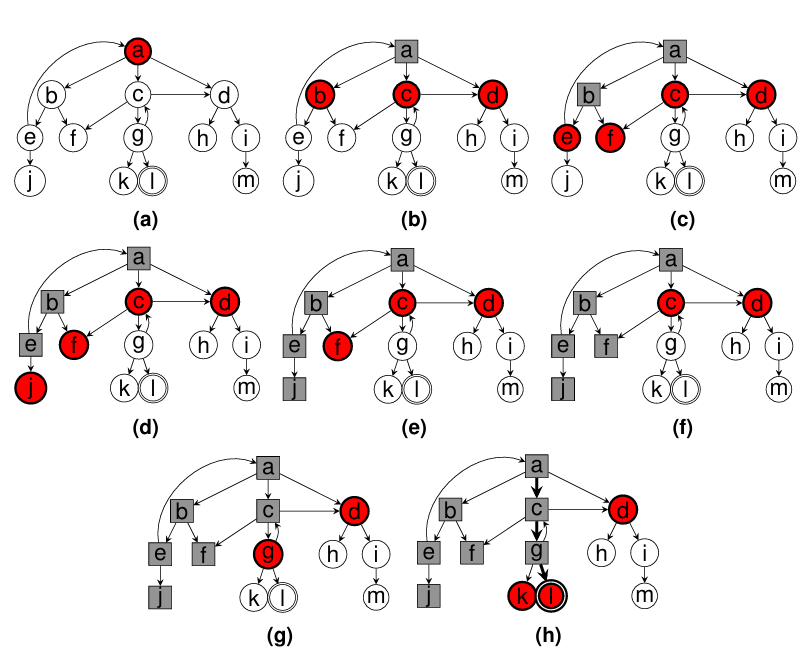
\includegraphics[width=0.8\textwidth]{./imgs/dfs.png}
	\caption{Depth First Search}
\end{figure}

\subsubsection{Pseudocode}
\begin{algorithm}[H]
	\caption{Depth First Search (\textit{start, goal})}\label{alg:dfs}
	\begin{algorithmic}[1]
		\State stack \(\gets\) [start]
		\While {stack is not empty}
		\State node \(\gets\) pop(stack)
		\If {node = goal}
		\State return path
		\EndIf
		\ForAll {neighbor in valid moves}
		\If {neighbor not visited}
		\State mark neighbor as visited
		\State push(stack, neighbor)
		\EndIf
		\EndFor
		\EndWhile
		\State return failure
	\end{algorithmic}
\end{algorithm}

\subsubsection{Implementation}
\begin{itemize}
	\item \textbf{\_\_init\_\_(\ldots)}
	      Initializes the DFS algorithm with grid dimensions, matrix representation, initial player position, stone positions, and switch positions. It also includes an optional deadlock detection flag.

	\item \textbf{search()}
	      Implements the DFS algorithm using a stack (LIFO). The search begins with the initial state in the frontier. The function explores states by popping from the stack and checking for the goal condition. If a new valid state is discovered, it is marked as visited and pushed onto the stack for further exploration.

	\item \textbf{can\_go(current\_state, dir)}
	      Checks whether the player can move in a given direction from the current state without encountering obstacles.

	\item \textbf{go(current\_state, dir)}
	      Generates a new state by moving the player in the specified direction, updating the relevant positions.

	\item \textbf{construct\_path(final\_state)}
	      Reconstructs the sequence of moves leading to the goal state by backtracking from the final state.

\end{itemize}


\subsubsection{Time and Space Complexity}
\textbf{Time Complexity:} \( O(b^m) \), where \( m \) is the maximum depth of the search tree. In the worst case, DFS may explore an entire path before backtracking.

\textbf{Space Complexity:} \( O(m) \), since DFS only needs to store nodes along the current path.
